\documentclass[10pt]{beamer}
\usetheme[
  titleformat=smallcaps
]{metropolis}

\usepackage{appendixnumberbeamer}
\usepackage{booktabs}
\usepackage[scale=2]{ccicons}
\usepackage{pgfplots}
\usepgfplotslibrary{dateplot}
\usepackage{xspace}
\usepackage[magyar]{babel}
\usepackage[export]{adjustbox}
\usepackage{fancybox}

\usepackage{graphicx}
\graphicspath{ {images/} }
\newcommand{\graphicswidth}{0.9\textwidth}

\title{Programkód-generálás természetes \\
  nyelvből mély neuronhálók használatával}
\date{2021. január 22.}
\author{Dina Tamás Pál~\inst{1} \hspace{0.2cm}\and Várkonyi Teréz Anna~\inst{2}}
\institute[Universities Here and There] {
  \vspace{0.4cm}
  \inst{1} ~Szerző - programtervező informatikus BSc
  \vspace{-0.2cm} \and
  \inst{2} ~Témavezető - egyetemi adjunktus, PhD}
\titlegraphic{\hfill
\includegraphics[height=1.5cm]{elte.png}}

\makeatletter
\setlength{\metropolis@progressonsectionpage@linewidth}{1pt}
\makeatother
\setbeamertemplate{section in toc}[sections numbered]
\hypersetup{pdfstartview={Fit}}
\metroset{titleformat title=regular}
\metroset{block=fill}

\begin{document}

\maketitle

\begin{frame}{Bevezetés}
  A dolgozatom \textbf{programozási feladatok automatikus megoldásával} foglalkozik, azon belül is a természetes nyelven alapuló programszintézis kérdésével.
  \begin{itemize}
    \item Dinamikusan fejlődő terület.
    \item Hatalmas elméleti és ipari potenciál.
    \item Interdiszciplináris: MI, formális nyelvek, számításelmélet.
  \end{itemize}
\end{frame}

\begin{frame}{Feladat}
  \begin{block}{Szemantikai elemzés}
    A szemantikai szövegelemzés feladata \textbf{természetes nyelvű lekérdezésekhez} (natural language query, NLQ) \textbf{formális jelentésreprezentációk} (formal meaning representation, FMR) párosítását jelenti.
  \end{block}
  \textbf{Formálisan}: Keressük a $\varphi \subseteq NLQ \times FMR$ relációt, amely adott $q = w_{1} ... w_{|q|} \in NLQ$ szósorozathoz egy adott formális nyelv szerinti $r = s_{1} ... s_{|r|} \in FMR$ terminális szimbólumok szekvenciáját rendeli.
\end{frame}

\begin{frame}{Feladat}
  \begin{block}{Intenció elemzés}
    A programíráskor végbemenő szemantikai tranzíció modellje.
  \end{block}
  A \textit{"feladat"}, \textit{"program"} és \textit{"megoldás"} fogalmak implicit kerülnek definiálásra a $(q, r) \in \varphi$ párok segítségével.
\end{frame}

\begin{frame}{Program áttekintése}
  \textbf{SASN: Simple Abstract Syntax Parser} \\
  Parancssori alkalmazás Docker konténerképként csomagolva.
  \begin{center}
    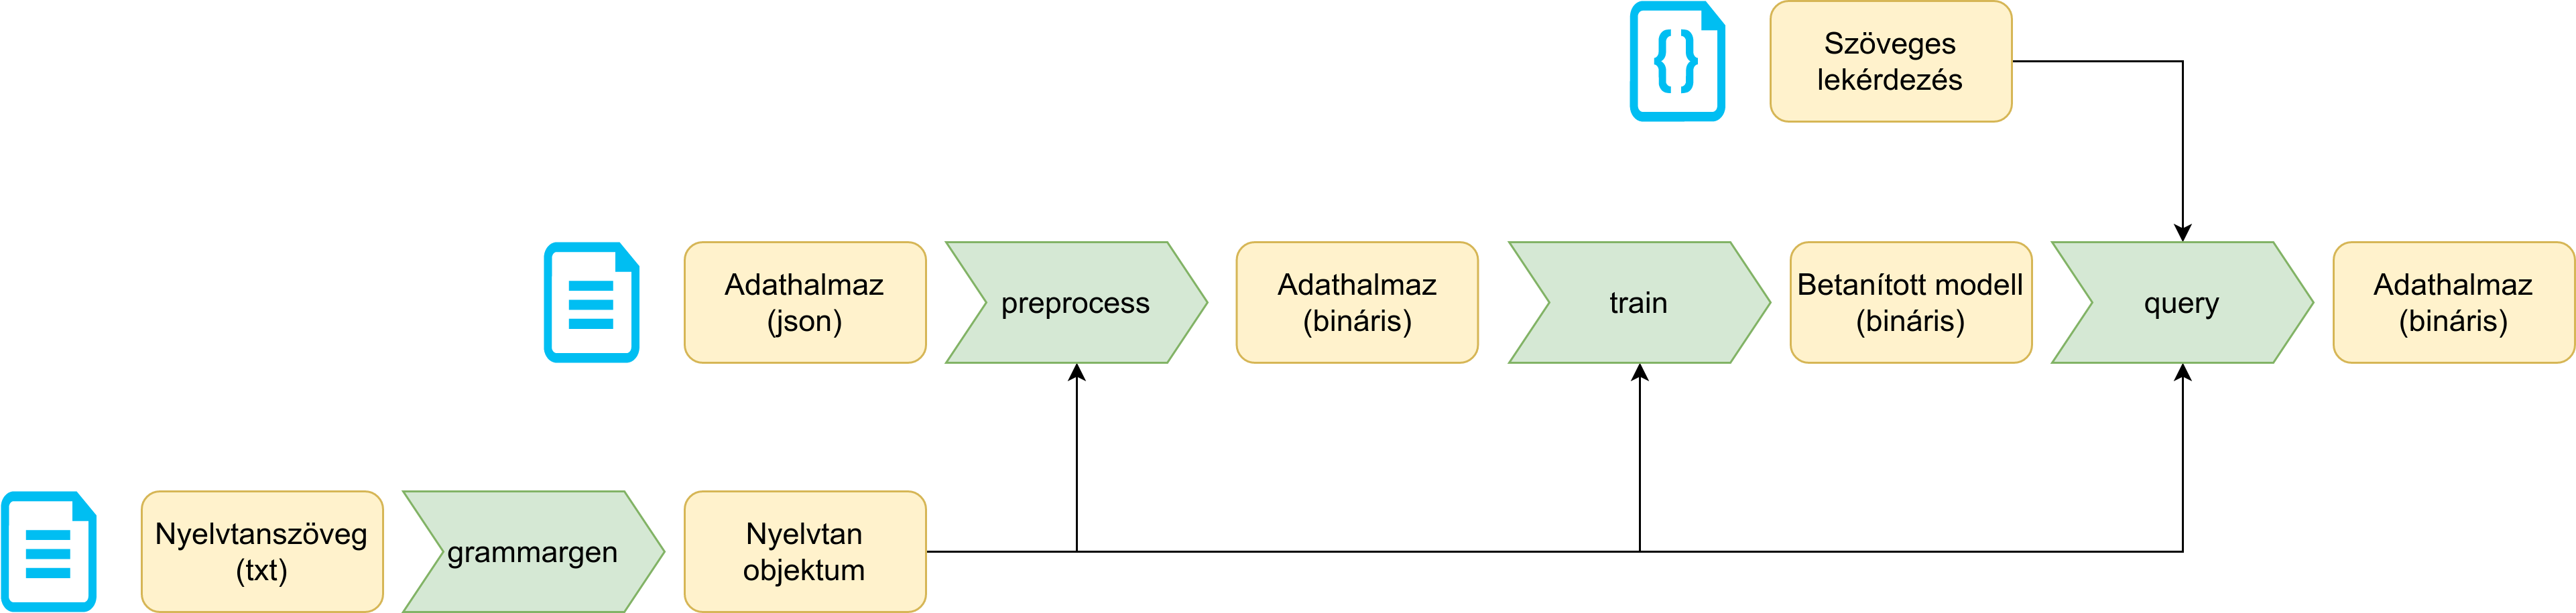
\includegraphics[width=9cm]{process.png}
  \end{center}
\end{frame}

\begin{frame}{Alkalmazott technikák}
  \begin{columns}[T]
    \column{0.5\textwidth}
    \textbf{Természetes szövegfeldolgozás:}
    \vspace{0.2cm}
    \begin{itemize}
      \item gépi tanulás
      \item statikus szókincs
      \item dinamikus szókiválasztás
      \item probabilisztikus modell
    \end{itemize}
    \column{0.5\textwidth}
    \textbf{Programkód-generálás:}
    \vspace{0.2cm}
    \begin{itemize}
      \item lexika, szintaxis
      \item fordítóprogram frontend
      \item köztes reprezentációk
      \item nemterminálisok generálása
    \end{itemize}
  \end{columns}
\end{frame}

\begin{frame}{Nyelvtani modul}
  A dolgozatom fő kontribúciója egy \textbf{automatizált nyelvtani modul}.\\
  De a rendszer tartalmaz egy neurális háló implementációt is.
  \begin{center}
    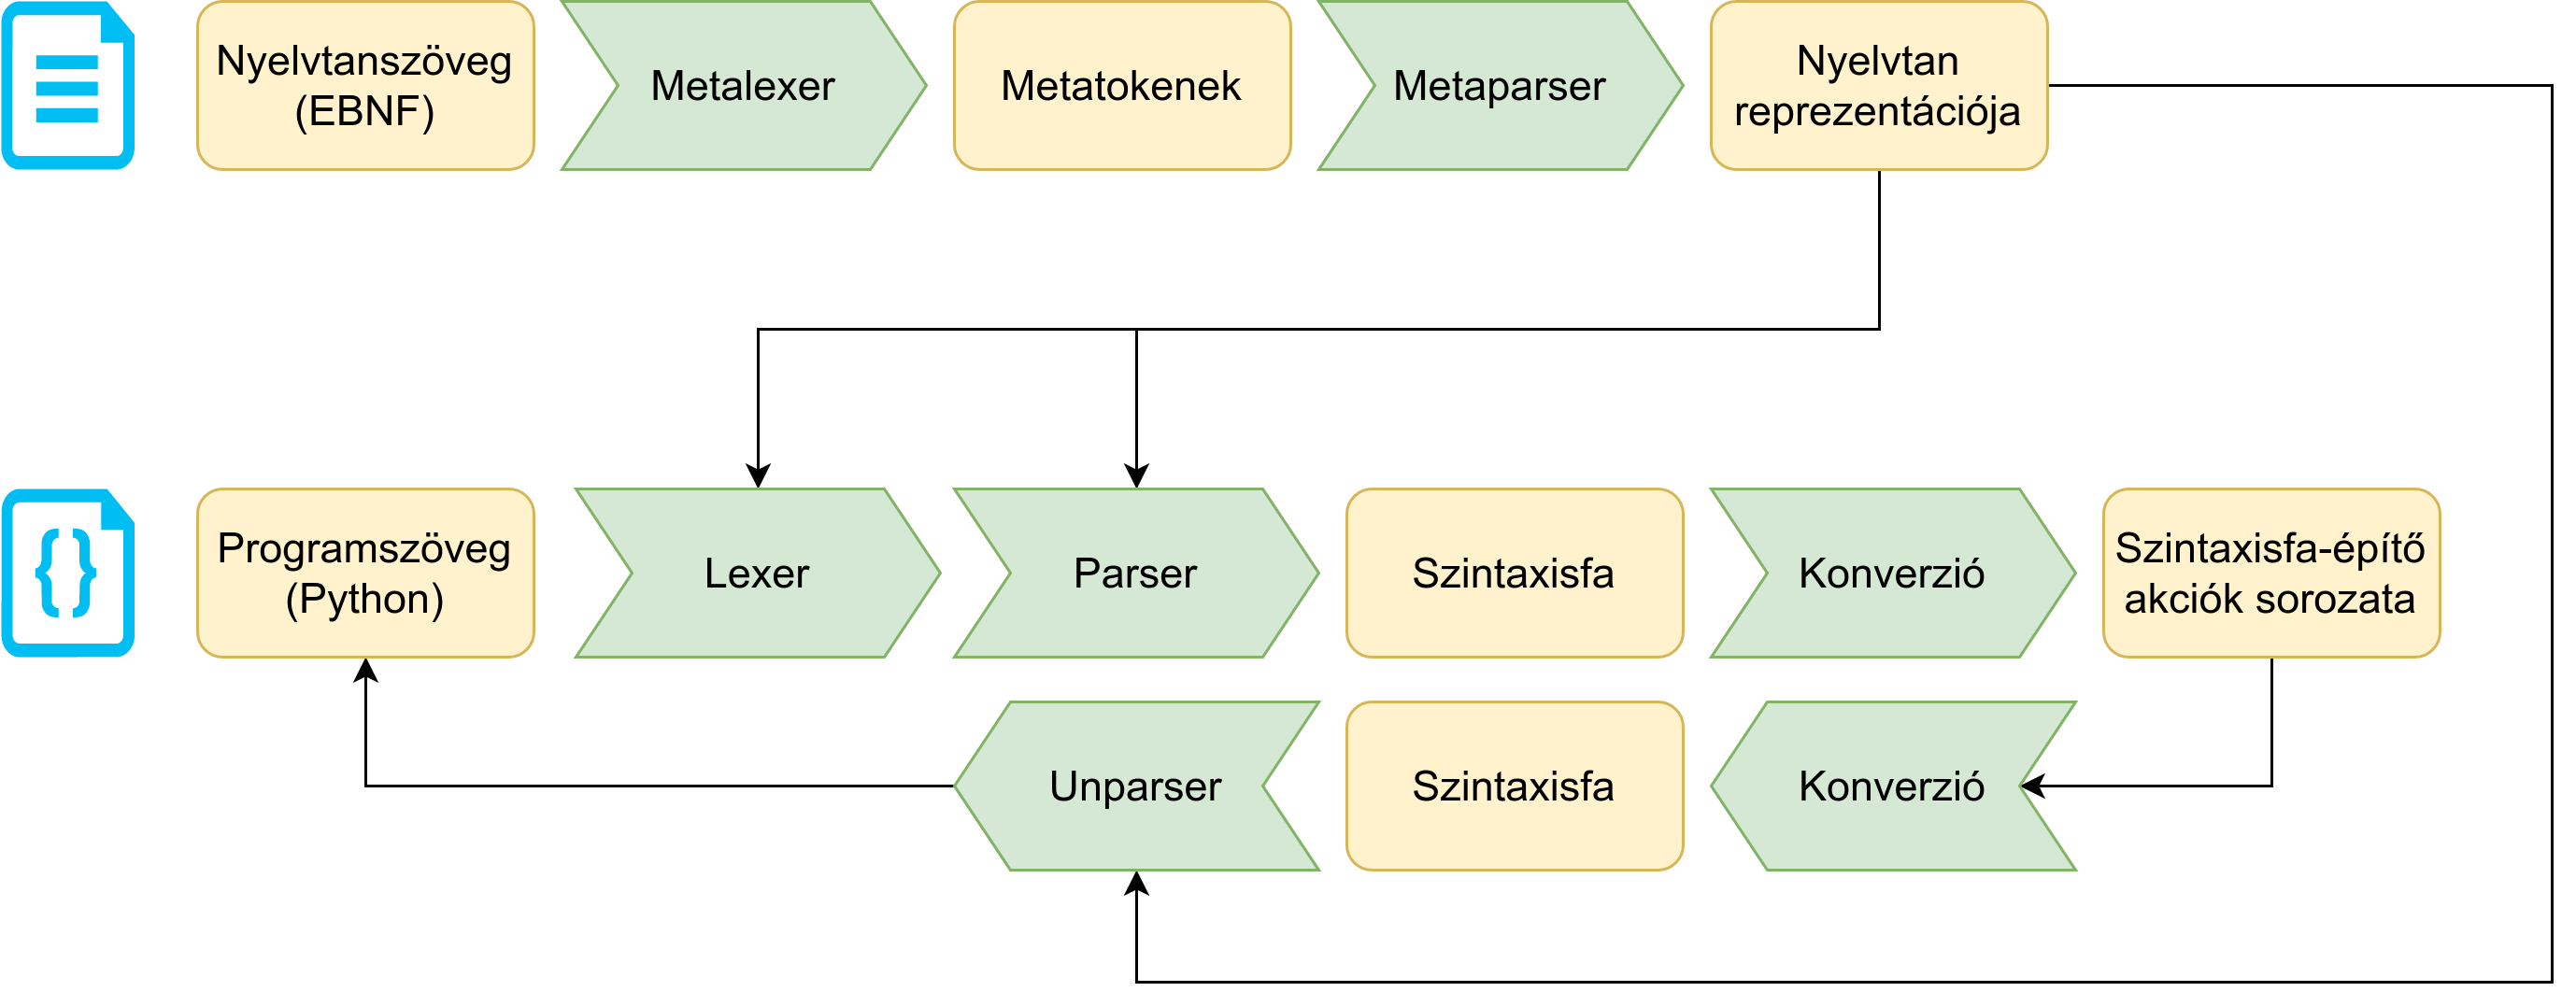
\includegraphics[width=8cm]{grammar.png}
  \end{center}
\end{frame}

\begin{frame}{Köztes reprezentációk}
  \begin{columns}[T]
    \column{0.5\textwidth}
    \begin{center}
      \textbf{Parciális szintaxisfa}
    \end{center}
    \vspace{0.2cm}
    \begin{center}
      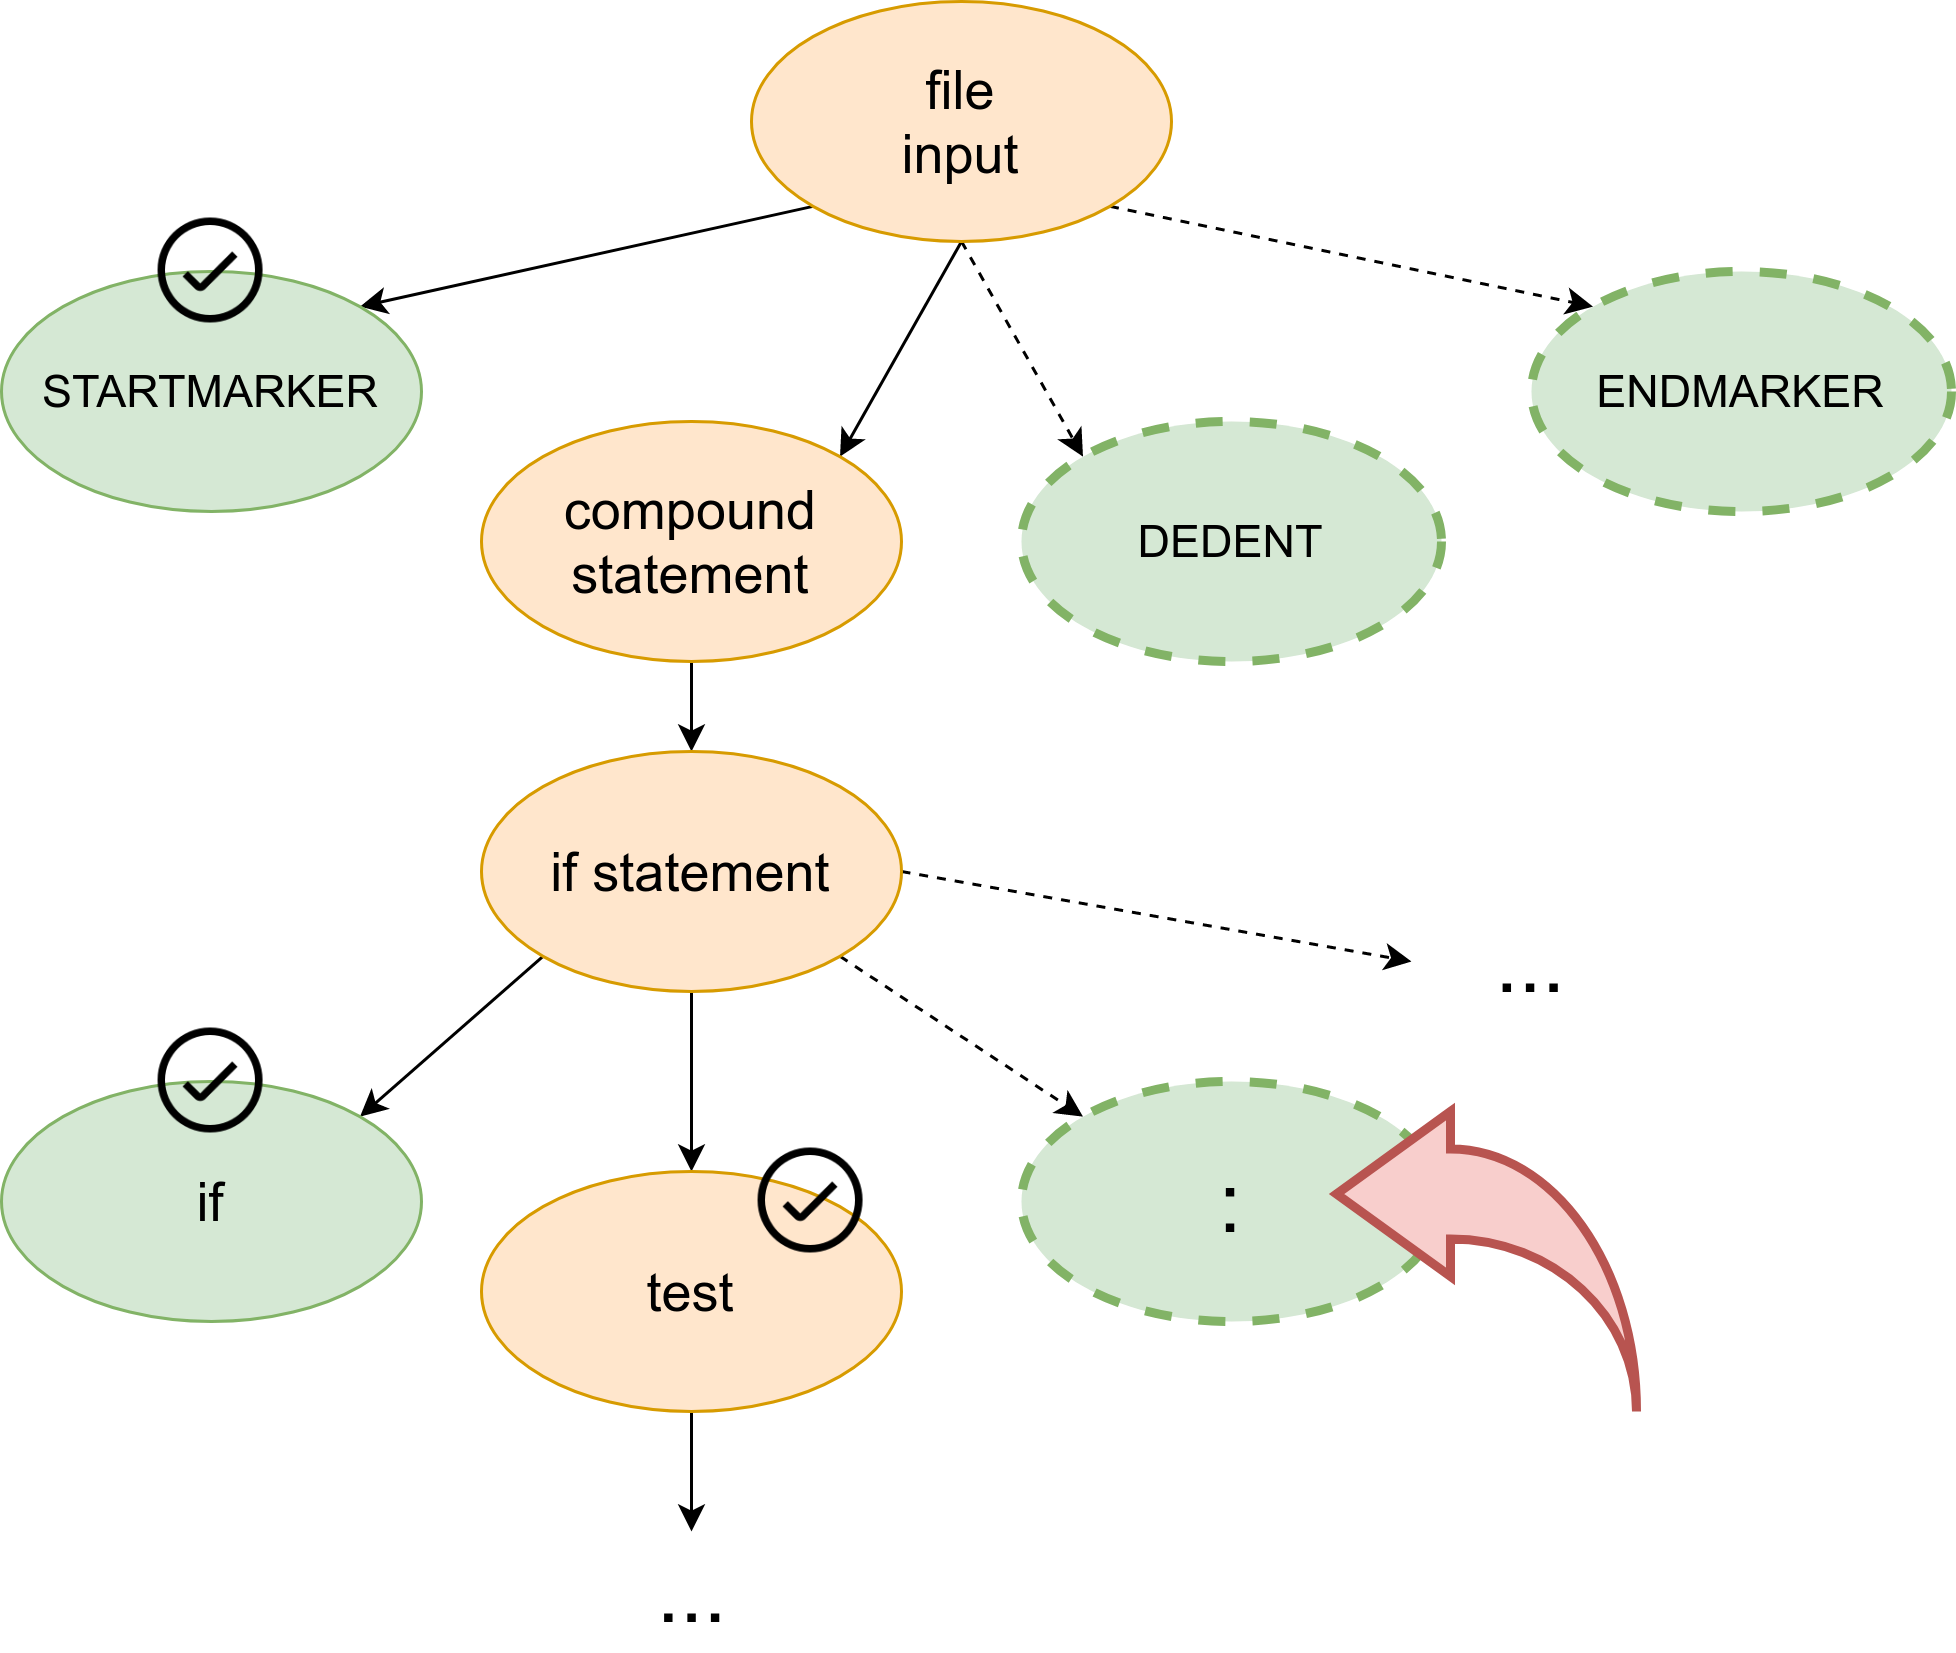
\includegraphics[width=5cm]{syntax_tree.png}
    \end{center}
    \column{0.5\textwidth}
    \begin{center}
      \textbf{Preorder építő algoritmus}
    \end{center}
    \vspace{0.2cm}
    \begin{center}
      \renewcommand{\arraystretch}{0.85}
      \begin{tabular}{ll}
      \toprule
      Akció & Paraméter\\
      \midrule
      \small\textsc{ApplyRule} & \footnotesize\texttt{file\_input}\\
      \small\textsc{GenToken}  & \footnotesize\texttt{startmarker}\\
      \small\textsc{Reduce}    & \footnotesize\texttt{-}\\
      \small\textsc{ApplyRule} & \footnotesize\texttt{compound\_stmt}\\
      \small\textsc{ApplyRule} & \footnotesize\texttt{if\_stmt}\\
      \small\textsc{GenToken}  & \footnotesize\texttt{'if'}\\
      \small\textsc{Reduce}    & \footnotesize\texttt{-}\\
      \multicolumn{2}{c}{...} \\
      \bottomrule
    \end{tabular}
    \end{center}
  \end{columns}
\end{frame}

\begin{frame}{Metanyelvtan}
  \begin{center}
    \shadowbox{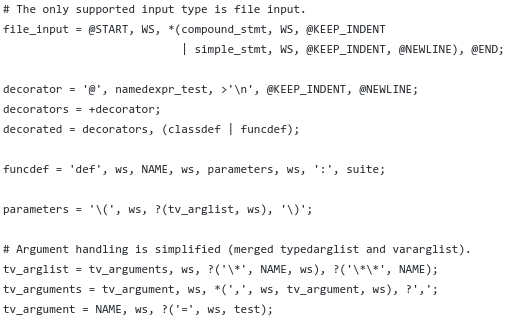
\includegraphics[width=8cm]{metagrammar.png}}
  \end{center}
\end{frame}

\begin{frame}{Metanyelvtan}
  \begin{center}
    \shadowbox{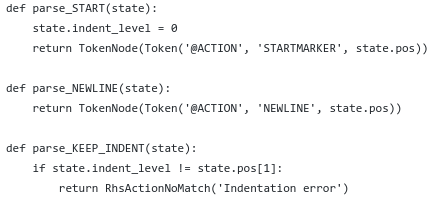
\includegraphics[width=8cm]{metagrammar_actions.png}}
  \end{center}
\end{frame}

\begin{frame}{Heurisztika}
  \begin{block}{Megoldó algoritmus}
    A megoldó algoritmus egy szekvencia-párosító rekurrens \\ \textbf{neurális háló} kódoló és dekódoló komponensekkel.
  \end{block}
  A modell tetszőlegesen bővíthető például neurális figyelemmel, dinamikus szómásolással, megerősített visszacsatolásokkal.
\end{frame}

\begin{frame}{Komponensek}
  \begin{itemize}
  \item Adathalmazok:
      \begin{itemize}
        \item nyelvtanfájl
        \item adatfájlok
        \item konfigurációs fájl
        \item generált parser/unparser modulok
      \end{itemize}
    \item Főprogram:
      \begin{itemize}
        \item metanyelvtan parser
        \item parser/unparser genetárok
        \item nyelvtani segédmodulok
        \item szintaxisfa-kezelő
        \item akciósorozat-kezelő
      \end{itemize}
  \end{itemize}
\end{frame}

\begin{frame}[standout]
  Köszönöm a figyelmet!
\end{frame}

\end{document}
